% !TeX spellcheck = en_GB
\documentclass[usenames,dvipsnames,aspectratio=169]{beamer}
\usetheme{Szeged}
\usecolortheme{beaver}
\setbeamertemplate{navigation symbols}{}
\usepackage{xcolor}

% \addbibresource{../VorlageAbschlussarbeit/Vorlage-Abschlussarbeit/Abschlussarbeit.bib}


\title{Web Processing - Standardized GIS Analyses for Cable Route Planning}
\author{Sebastian Heiden}
\institute{Harz University of Applied Sciences}
\date{October 14, 2022}
\begin{document}

    

\begin{frame}[plain]
	
\includegraphics[scale=0.21]{images/3-HSH-Logo-RGB-en.png}
    \maketitle
\end{frame}
%\begin{frame}{Structure}
%    \tableofcontents    
%\end{frame}

\section{Topic and Motivation}
\begin{frame}{Topic and Motivation}
\begin{columns}[T] % align columns
\begin{column}{.68\textwidth}
	Topic
	\begin{itemize}
		\item route planning, e.g. connection of offshore wind farms to the power grid
		\item conflicts with land usage, land coverage, regulation
		\item routing cables from landing point to final position
		\item offer a standard web service for the routing

	\end{itemize}
	\vspace{0.5cm}
	Motivation
	\begin{itemize}
		\item Energy Security
		\item Contribution to important real world problems
	\end{itemize}
\end{column}%
\hfill
\begin{column}{.28\textwidth}
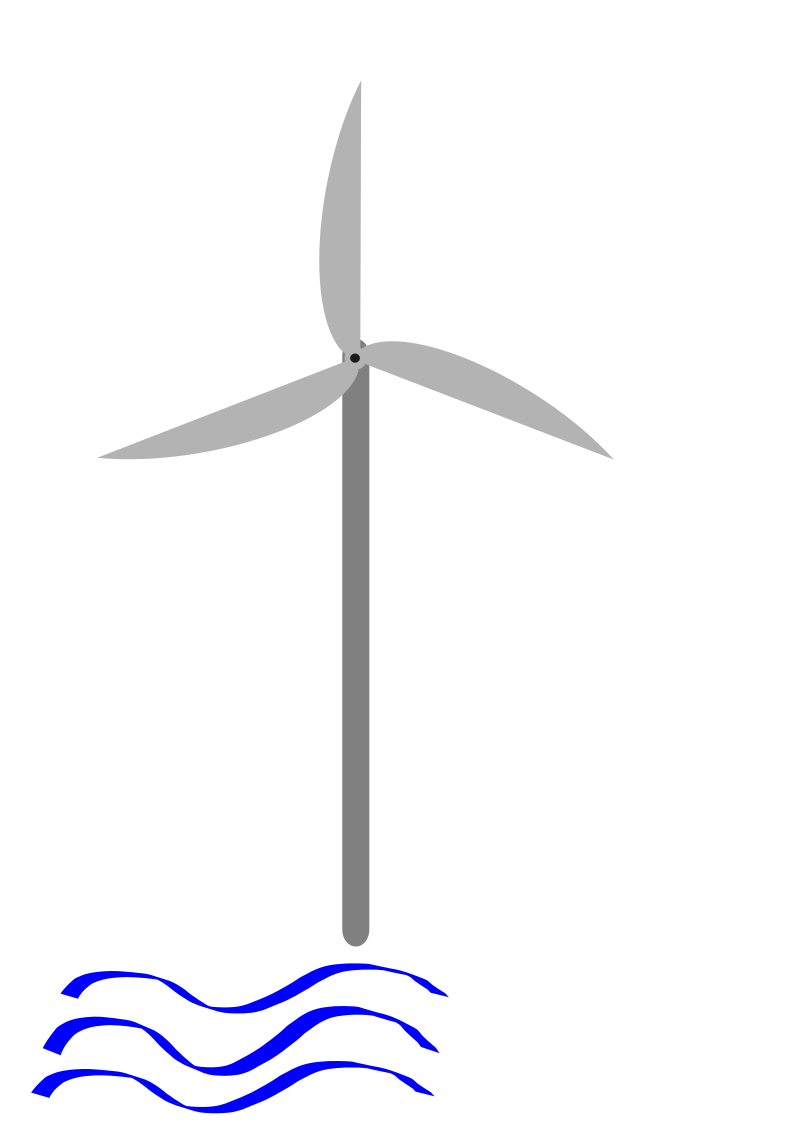
\includegraphics[scale=0.2]{images/icon_offshore_wind_turbine.png}
\end{column}%
\end{columns}
\end{frame}

\section{Method and Research Issue}
\begin{frame}{Method and Research Issue}
	Method
	\begin{itemize}
		\item Least cost path (LCP)
		\begin{enumerate}
			\item input: Destination and Cost Raster
		%\item Computes: Aggregated Cost Raster/ Backlink Raster
			\item Aggregated Cost and Backlink $\rightarrow$ Route
		\end{enumerate}
		\item Web Processing Service (WPS)
		\begin{itemize}
			\item standardized GIS\footnote{Geographic information system} web service
			\item processing spatial data (Raster and Vector)
		\end{itemize}
	\end{itemize}
Research Issue
\begin{itemize}
\item optimization of rasterization
\item reduce area of high resolution raster
\end{itemize}
\end{frame}

\section{Timetable}
\begin{frame}{Timetable}
\begin{center}
	\begin{small}
	\begin{tabular}{ | c | c | l| }
		\hline
		Start Date & End Date &  \\ 
		\hline\hline
		09/23/2022 & 					& \color{gray}{Project Start}\\
		09/23/2022 & 10/10/2022 	& \color{gray}{Initial Literature Study}\\
		10/01/2022 & 10/23/2022 	& \color{gray}{Initial Data Search}\\
		\hline
		10/14/2022 & 					& Kick-Off Presentation\\
		\hline

		10/16/2022 & 10/28/2022 	& Data Conversion/Costs/test execution\\
		10/28/2022 & 12/31/2022 	& provide WPS/implement LCP\\
		\hline
		12/14/2022 & 					& Midterm  Presentation\\
		\hline
		12/14/2022 & 02/01/2022 	& Optimization/Research Issue\\
		02/01/2022 & 					& Feature Freeze \\ 
		02/01/2022 & 02/28/2023 	& Finalizing Report\\ 
		\hline
		02/28/2023 & 					& Submission  \\
		03/15/2023 & 					& Final Presentation  \\
		\hline   
	\end{tabular}
	\end{small}
\end{center}
\end{frame}


\end{document}
